
\documentclass[12pt]{article}
\usepackage{graphicx} % for including images
\usepackage{hyperref} % for creating hyperlinks
\usepackage{amsmath} % for mathematical expressions
\usepackage{lipsum} % for generating dummy text
\usepackage{listings} % for code blocks
\usepackage{float} % place images where they appear in the LaTeX
\usepackage{pdfpages} % insert PDFs in the document

\lstset{
  language=bash,
  basicstyle=\ttfamily,
  breaklines=true
}

\begin{document}
% Title page information
\title{Sound Classification and Localization by Acoustic Sensing on Raspberry Pi 4}
\author{Jaidon Lybbert, University of Washington}
\date{January 24, 2024}

% Generate the title page
\maketitle

% Abstract section
\begin{abstract}
	In this article a network of distributed acoustic sensing nodes is used to localize a sound signature using a time-difference-of-arrival (TDoA) algorithm. Accurate wall-clock times are obtained by GPS at each node, and a frame of acoustic data is recorded through a microphone on each node. Time differences are determined by correlation, and the resulting system of equations solved by the Chan-Ho algorithm to determine location. In a concurrent process, each node performs classification inference on a data frame using a pre-trained convolutional neural network (CNN). The resulting class identification is used to assign a process model to the tracked object for use in an Extended Kalman Filter (EKF) applied to the Chan-Ho localization result to make the final estimate of object position and trajectory.
\end{abstract}


% Methods section
\section{Background}\label{sec:background}

Bird watchers have developed software tools for collecting data around the world about bird activity. One of the larger projects is BirdNET, a machine learning model for classifying bird species by sound. Hardware projects exist to listen to the environment and use BirdNET to classify bird species and upload the results to BirdWeather, a database of detections of bird species around the world. One of these projects is BirdNET-Pi which does this on the Raspberry Pi. 

Detected bird activity is associated with the GPS coordinates of the sensing device. On the Raspberry Pi, which doesn't have a GPS module, the coordinates are manually entered, or the coordinates entered automatically by the Raspberry Pi OS installation tool are used. As a result, the detected locations are very imprecise, on the order of 10s, 100s, or even 1000s of meters, depending on the diligence of the user. This is probably adequate for monitoring bird activity on a global scale.

My project seeks to localize detected birds with precision in the range of less than 1 meter in an area the size of a backyard. The goal is to know when and where in the backyard birds of different species can be spotted. 


\subsection{Project Architecture Overview}
	My project can be split into three major functions: data collection, classification, and localization. Classification requires one audio source, and localization requires at least 3 simultaneous audio sources for triangulating. To provide a simultaneuous reference clock, GPS units are used. 

\subsection{Environment Setup}

	My project consists of the following hardware:
\lstlisting{}
\item{Raspberry Pi 4B}
\item{Adafruit Feather Huzzah (ESP8266)}
\item{Adafruit Ultimate USB GPS breakout board}
\item{Breadboard}
\item{Jumper wires}
\item{Elegoo 3.3V breadboard power supply}
\item{2 x 100kOhm resistors}
\item{1 x 0.1uF capacitor}
\item{1 x 220Ohm resistor}
\item{1 x 3.3V electret microphone module}
	

\subsection{Data Collection}
Data collection consists of getting audio and GPS data onto the Raspberry Pi. The data from the sensor array is used by both the classifier and the localization algorithm to determine species and location. The audio data is first sensed by the electret microphone module, then filtered by an RC network, and sampled by the ESP8266 MCU. The ESP opens a web socket and listens for a connection from the Raspberry Pi, when the Raspberry Pi connects, the ESP begins streaming audio data over the socket until the connection is terminated.

\subsection{Classification}
For classification, and audio signal is recorded by a microphone in the environment, and the digital signal is interpreted by an algorithm to determine species. Classification consists of running inference on the data from the microphone to determine the species. Classification is done using a pre-trained machine-learning model from the BirdNET project. The model is loaded on the Raspberry Pi 4B using the TensorFlow Lite runtime. 

\subsection{Localization}
To localize something based on sound, an array of at least 3 spatially distributed microphones is used. Since the microphones have to be far apart from each other in an outdoor environment, it would be inconvenient to run long cables to each microphone. For this reason, I have opted to use a network of WiFi enabled ESP8266 MCUs to sample audio data and communicate the collected audio buffers to the Raspberry Pi through web sockets for performing the localization algorithm.

The localization algorithm is a two step process. In the first stage, the signal recieved by each pair of sensing nodes in the network is cross-correlated to find the Time-difference of Arrival (TDoA) between those two nodes. The TDoA defines a hyperbola in space, where the source could be located. Each sensor defines one more hyperbola in space. With 3 sensors, two hyperbolas are defined and the intersection gives two possible locations for the source. With more than 3 sensors, the system of equations is overdetermined, and a least-squares method is used. So, solving the system of equations can be considered the second step in the localization algorithm, after TDoA estimation.

For my project, I will be using the Generalized Cross-correlation Phase Transform (GCC-PHAT) algorithm for TDoA estimation, and the Chan-Ho algorithm for solving the system of equations.

\subsection{Simulation}
For initial verification of my localization algorithm to rapidly test under varying parameters, I created a simple simulator which takes an MP3 file, and performs transformations on it to add delay and noise to simulate the audio signal recieved by the network of sensor nodes. The simulated signals are then fed into the TDoA and Chan-Ho algorithm to estimate source location. A graphical user interface using Pygame shows the geometry of the sensors and source, and displays the error in position estimate and a bounding box over the true location.

\section{Methods}\label{sec:methods}
\subsection{TensorFlow Lite}
	
	TensorFlow Lite (TFLite) is a lightweight version of the TensorFlow runtime for loading machine learning models and running inference on input data. TFLite runs on resource-constrained devices like the Raspberry Pi. I use TFLite for loading a pretrained model for classification of bird species by sound. The model of choice is taken from the BirdNET project, and contains 6,000 species. The input to the model is a 3 second long frame of audio sampled at 48kS/s, and the output is an 6k element array containing the class estimates. The model has a secondary input which takes in latitude, longitude, and the week of the year (1-52).
	
	I first referenced the TFLite Python API documentation to attempt loading the model, and running it against a sample audio clip. I quickly found out that the high-level API and provided binaries for the \textbf{aarch64} architecture are not well supported by the TensorFlow developers. I shifted my strategy to setting up the BirdNET-Pi project to run on my device. I ran into build and dependency issues, since the developers of the BirdNET-Pi project support a previous release of the Raspberry Pi OS. Instead of re-installing a different OS, I used the source code of BirdNET-Pi as reference to write a minimally working script to get TFLite working on the Pi.
	
	The BirdNET model contains functions that require a piece of software to be compiled in with the TFLite binary. This runtime is not available in the binary provided by the TFLite developers, so I used a version provided by an independent developer who compiles the runtime with this software for the Pi. The TFLite wheel was incompatible with the system installation of Python 3.11 included in the Raspberry Pi OS. I installed \textbf{pyenv} to install Python 3.9 and manage the two different versions. The versions of packages required by the TFLite wheel, such as \textbf{Numpy} were incompatible with the versions installed by \textbf{pip} by default, and changing the version manually broke dependency rules for other packages like \textbf{matplotlib}. I created a \textbf{requirements.txt} file for \text{pip}, and manually wrote the dependency rules  to get all packages working.
	
	I took a sample audio \textbf{MP3} of a known bird species from an online database, and loaded it into Python with \textbf{pydub}, and converted it to a \textbf{Numpy} array. I wrote a function to split the file into 3 second chunks. For each chunk, I put the array of samples into the first TFLite input tensor, and put the location and time data into the second input tensor. I timed how long it took for inference, and recorded the estimate result. I plotted the inference execution time over all frames of audio.
	
\subsubsection{GPS}
	
	I used the Adafruit Ultimate GPS USB breakout board to get GPS data through \textbf{gpsd} \cite{townsend2023}. \textbf{gpsd} is a Linux daemon which listens on port 2497 of the loopback address by default. When a connection request is recieved, it begins communicating with the GPS module over USB by reading data through the /dev/ttyUSB0 device file, and forwarding it to the TCP/IP port to service the request. By default, \textbf{gpsd} is managed through \textbf{systemd}. Adafruit recommends disabling this functionality through the \textbf{systemctl} interface, and running \textbf{gpsd} manually.

\begin{figure}[h]
\centering
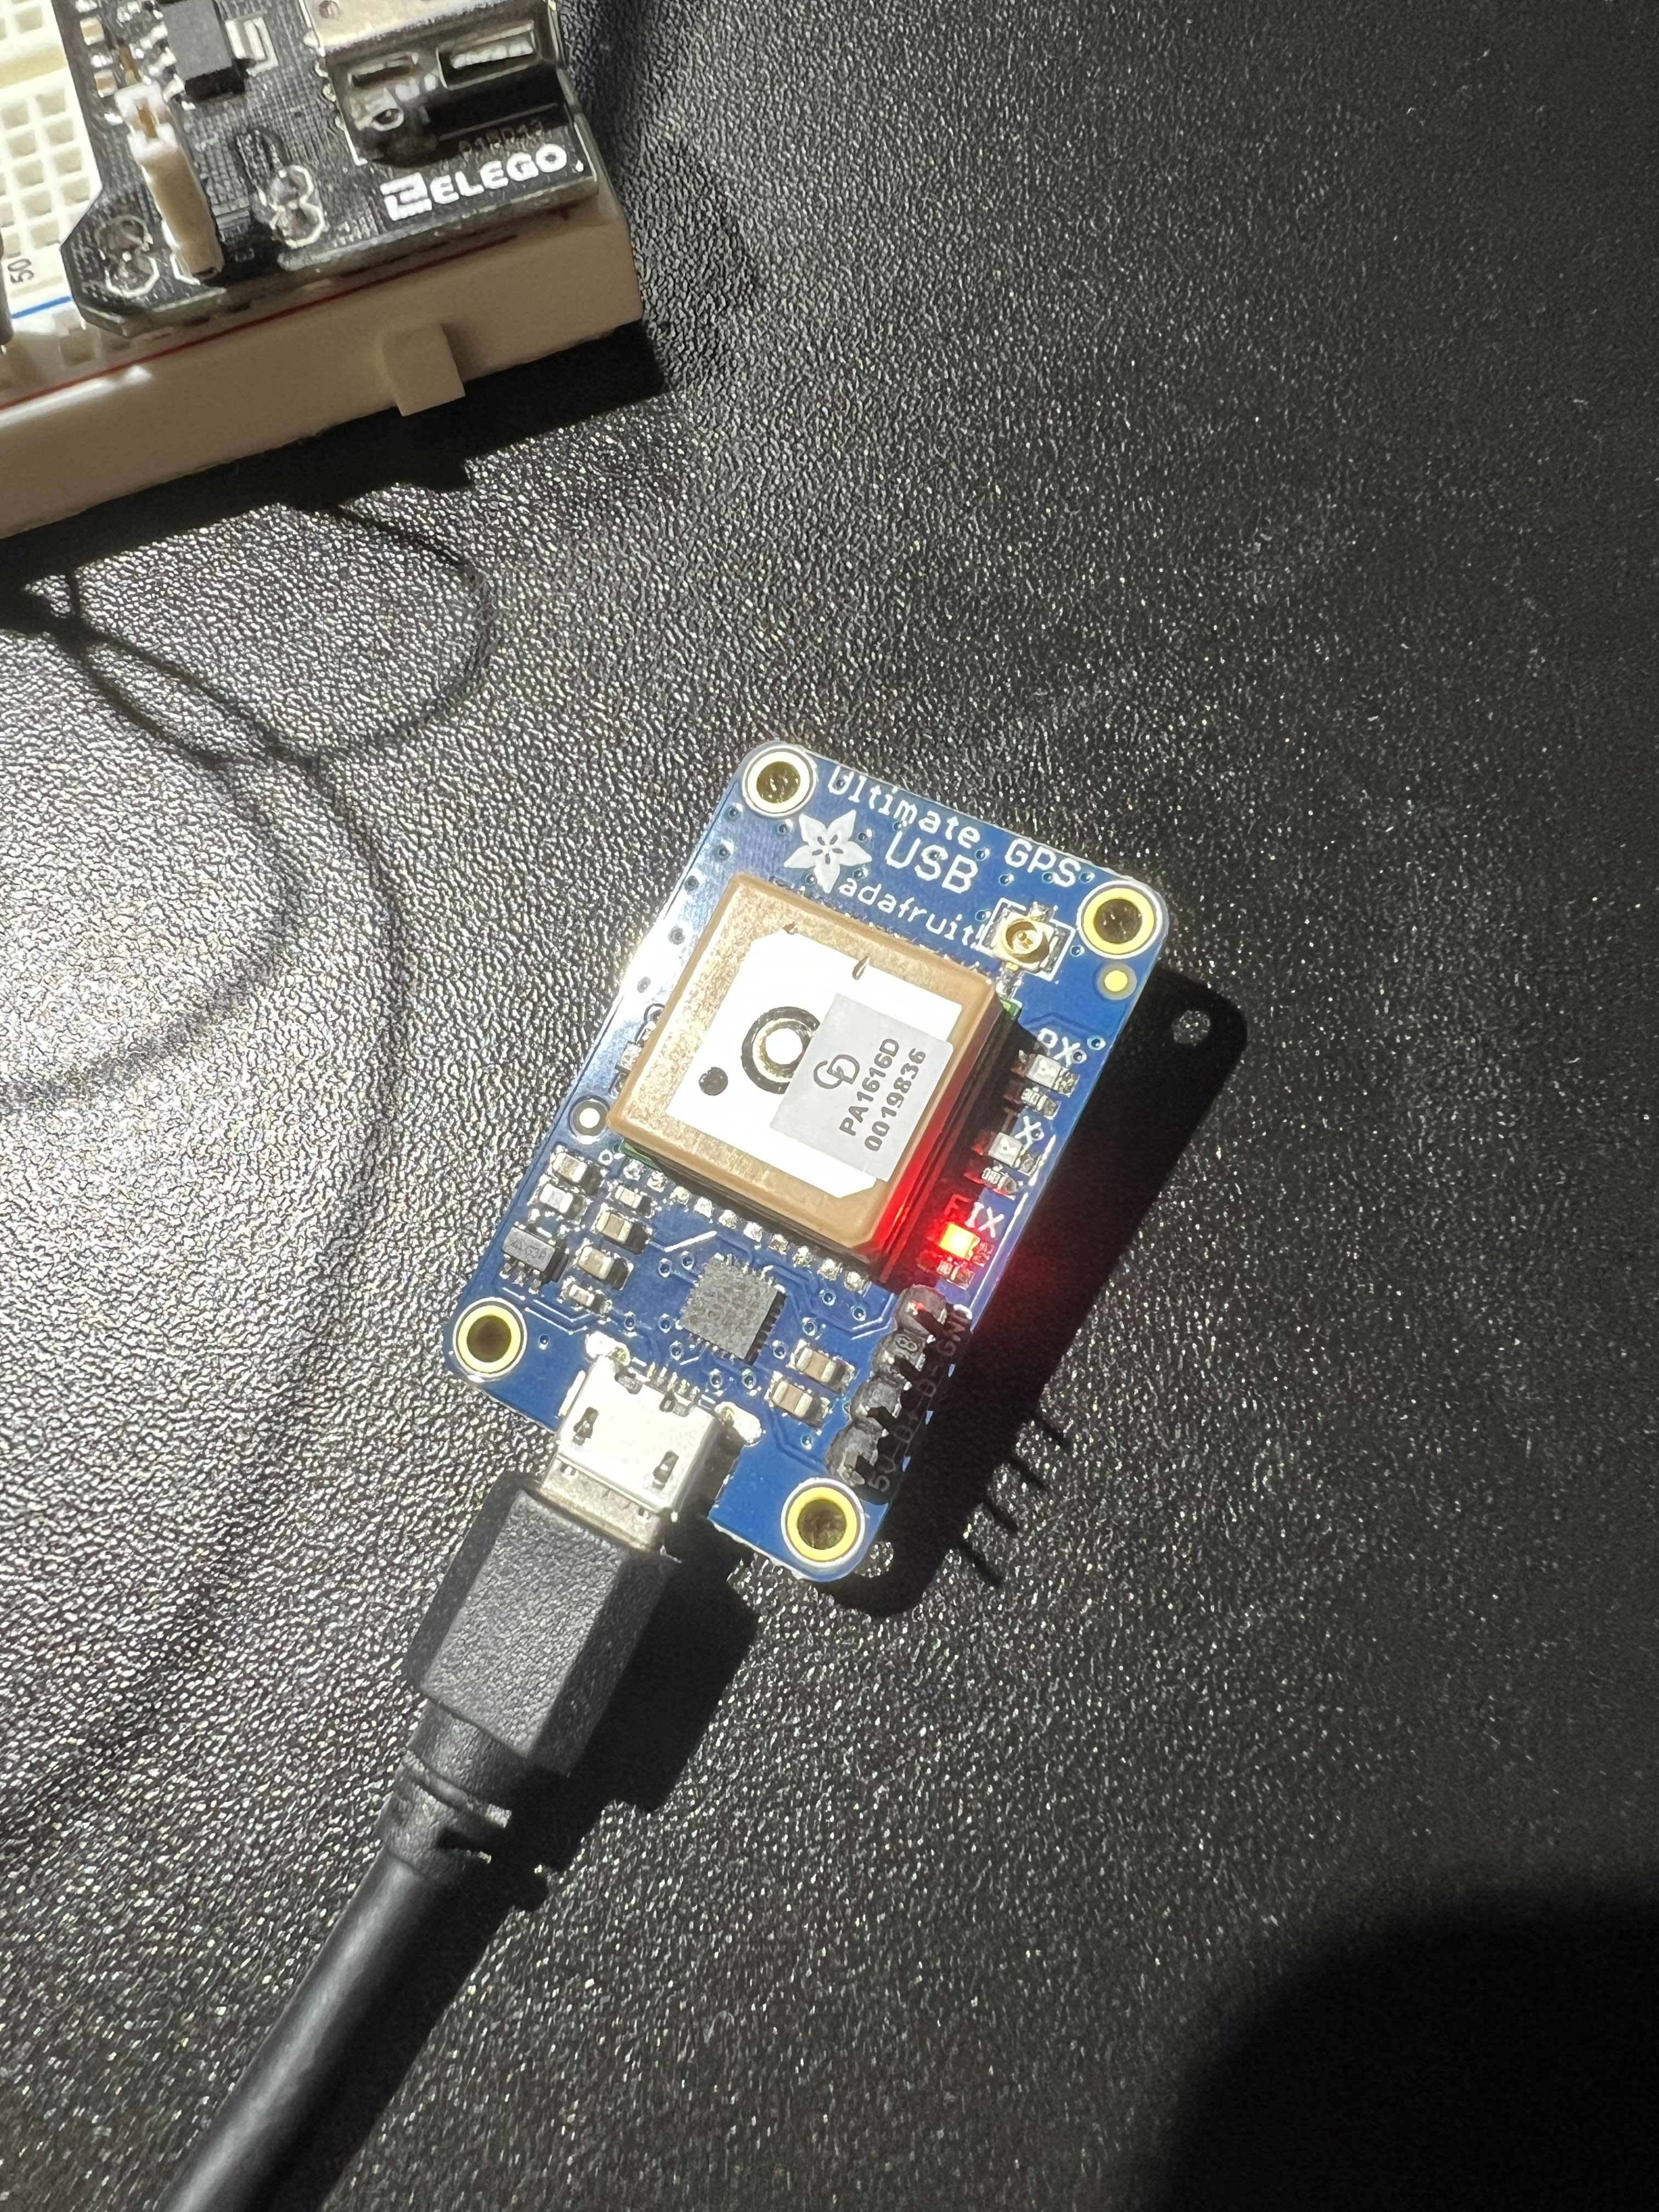
\includegraphics[width=0.8\textwidth]{gps_hardware.jpg} % replace with your own image file
\caption{Adafruit Ultimate USB GPS module. The device has an on-board serial-to-USB adapter, so the module can be plugged directly into a USB port on the Raspberry Pi 4B.}
\label{fig:gps_hardware}
\end{figure}
	
\begin{lstlisting}
sudo apt install gspd gpsd-clients
sudo systemctl stop gpsd.socket
sudo systemctl disable gpsd.socket
sudo killall gpsd
sudo gpsd /dev/ttyUSB0 -F /var/run/gpsd.sock
\end{lstlisting}

To test the device I used the command \textbf{cgps -s}, which is a \textbf{gspd} client that communicates over the default port and prints out GPS status information to the console, as shown in Fig. \ref{fig:cgps}. It took significant troubleshooting to get this to work properly. What I finally determined to work was editing the configuration of \textbf{gpsd} defined in the \textbf{/etc/default/gpsd} file, and rebooting. 

\begin{lstlisting}
DEVICES=""
START_DAEMON="true"
GPSD_OPTIONS="/dev/ttyUSB0 -G"
USBAUTO="true"
GPSD_SOCKET="/var/run/gpsd.sock"
\end{lstlisting}

The other necessary step was physically moving my test setup from the basement to the main floor of my house, since I could not get a reliable connection to the GPS satellites from the basement.

Once I had a reliable connection, I wrote a Python script to collect about 1200 GPS readings of latitude and longitude, while leaving the system stationary, and wrote the readings to a \textbf{.csv} file. I wrote a script to convert degrees of latitude and longitude to meters, then plotted a histogram of the differences of each reading from the mean value to evaluate the spatial precision of the GPS reciever.

\begin{figure}[h]
\centering
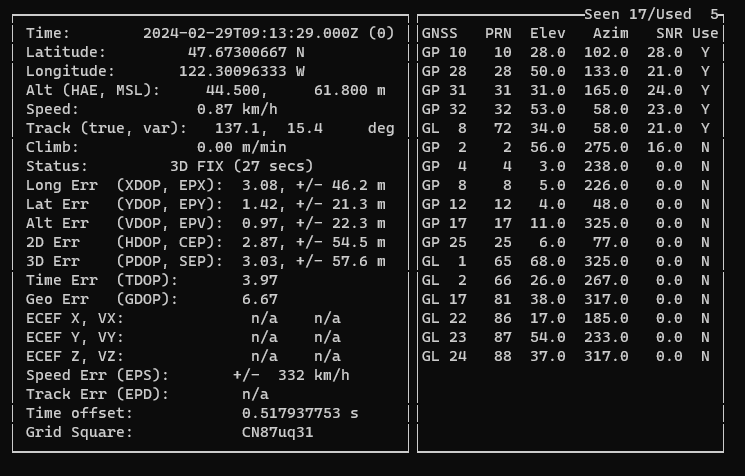
\includegraphics[width=0.8\textwidth]{cgps.png} % replace with your own image file
\caption{Terminal display of GPS information from the \textbf{cgps -s} command.}
\label{fig:cgps}
\end{figure}

\subsection{Microphone}
	I use an generic adjustable-gain microphone module to sample the acoustic signals with the ESP8266 sensing node. For my breadboard prototype, I don't have an ADC capable of sampling at the 48kS/s rate required by the TFLite model. Given more time, I would implement the Analog Devices SSM2603 audio CODEC, which has programmable gain and a digital I2S interface. 
	I power the microphone with 3.3V from an ELEGOO breadboard power supply connected to a wall outlet through a 9V wall wart. The microphone output is connected to a simple first-order low-pass antialiasing filter implemented with a resistor and capacitor on the breadboard with a cutoff frequency of 20kHz. The output of the filter is connected to an ADC on the ESP8266.
	To characterize the microphone noise, I tape over the transducer, then sample the ADC with the ESP8266, and send the samples over to the Raspberry Pi through the web socket interface. I record the samples to a \textbf{CSV} to plot the sample distribution.
	
\begin{figure}[h]
\centering
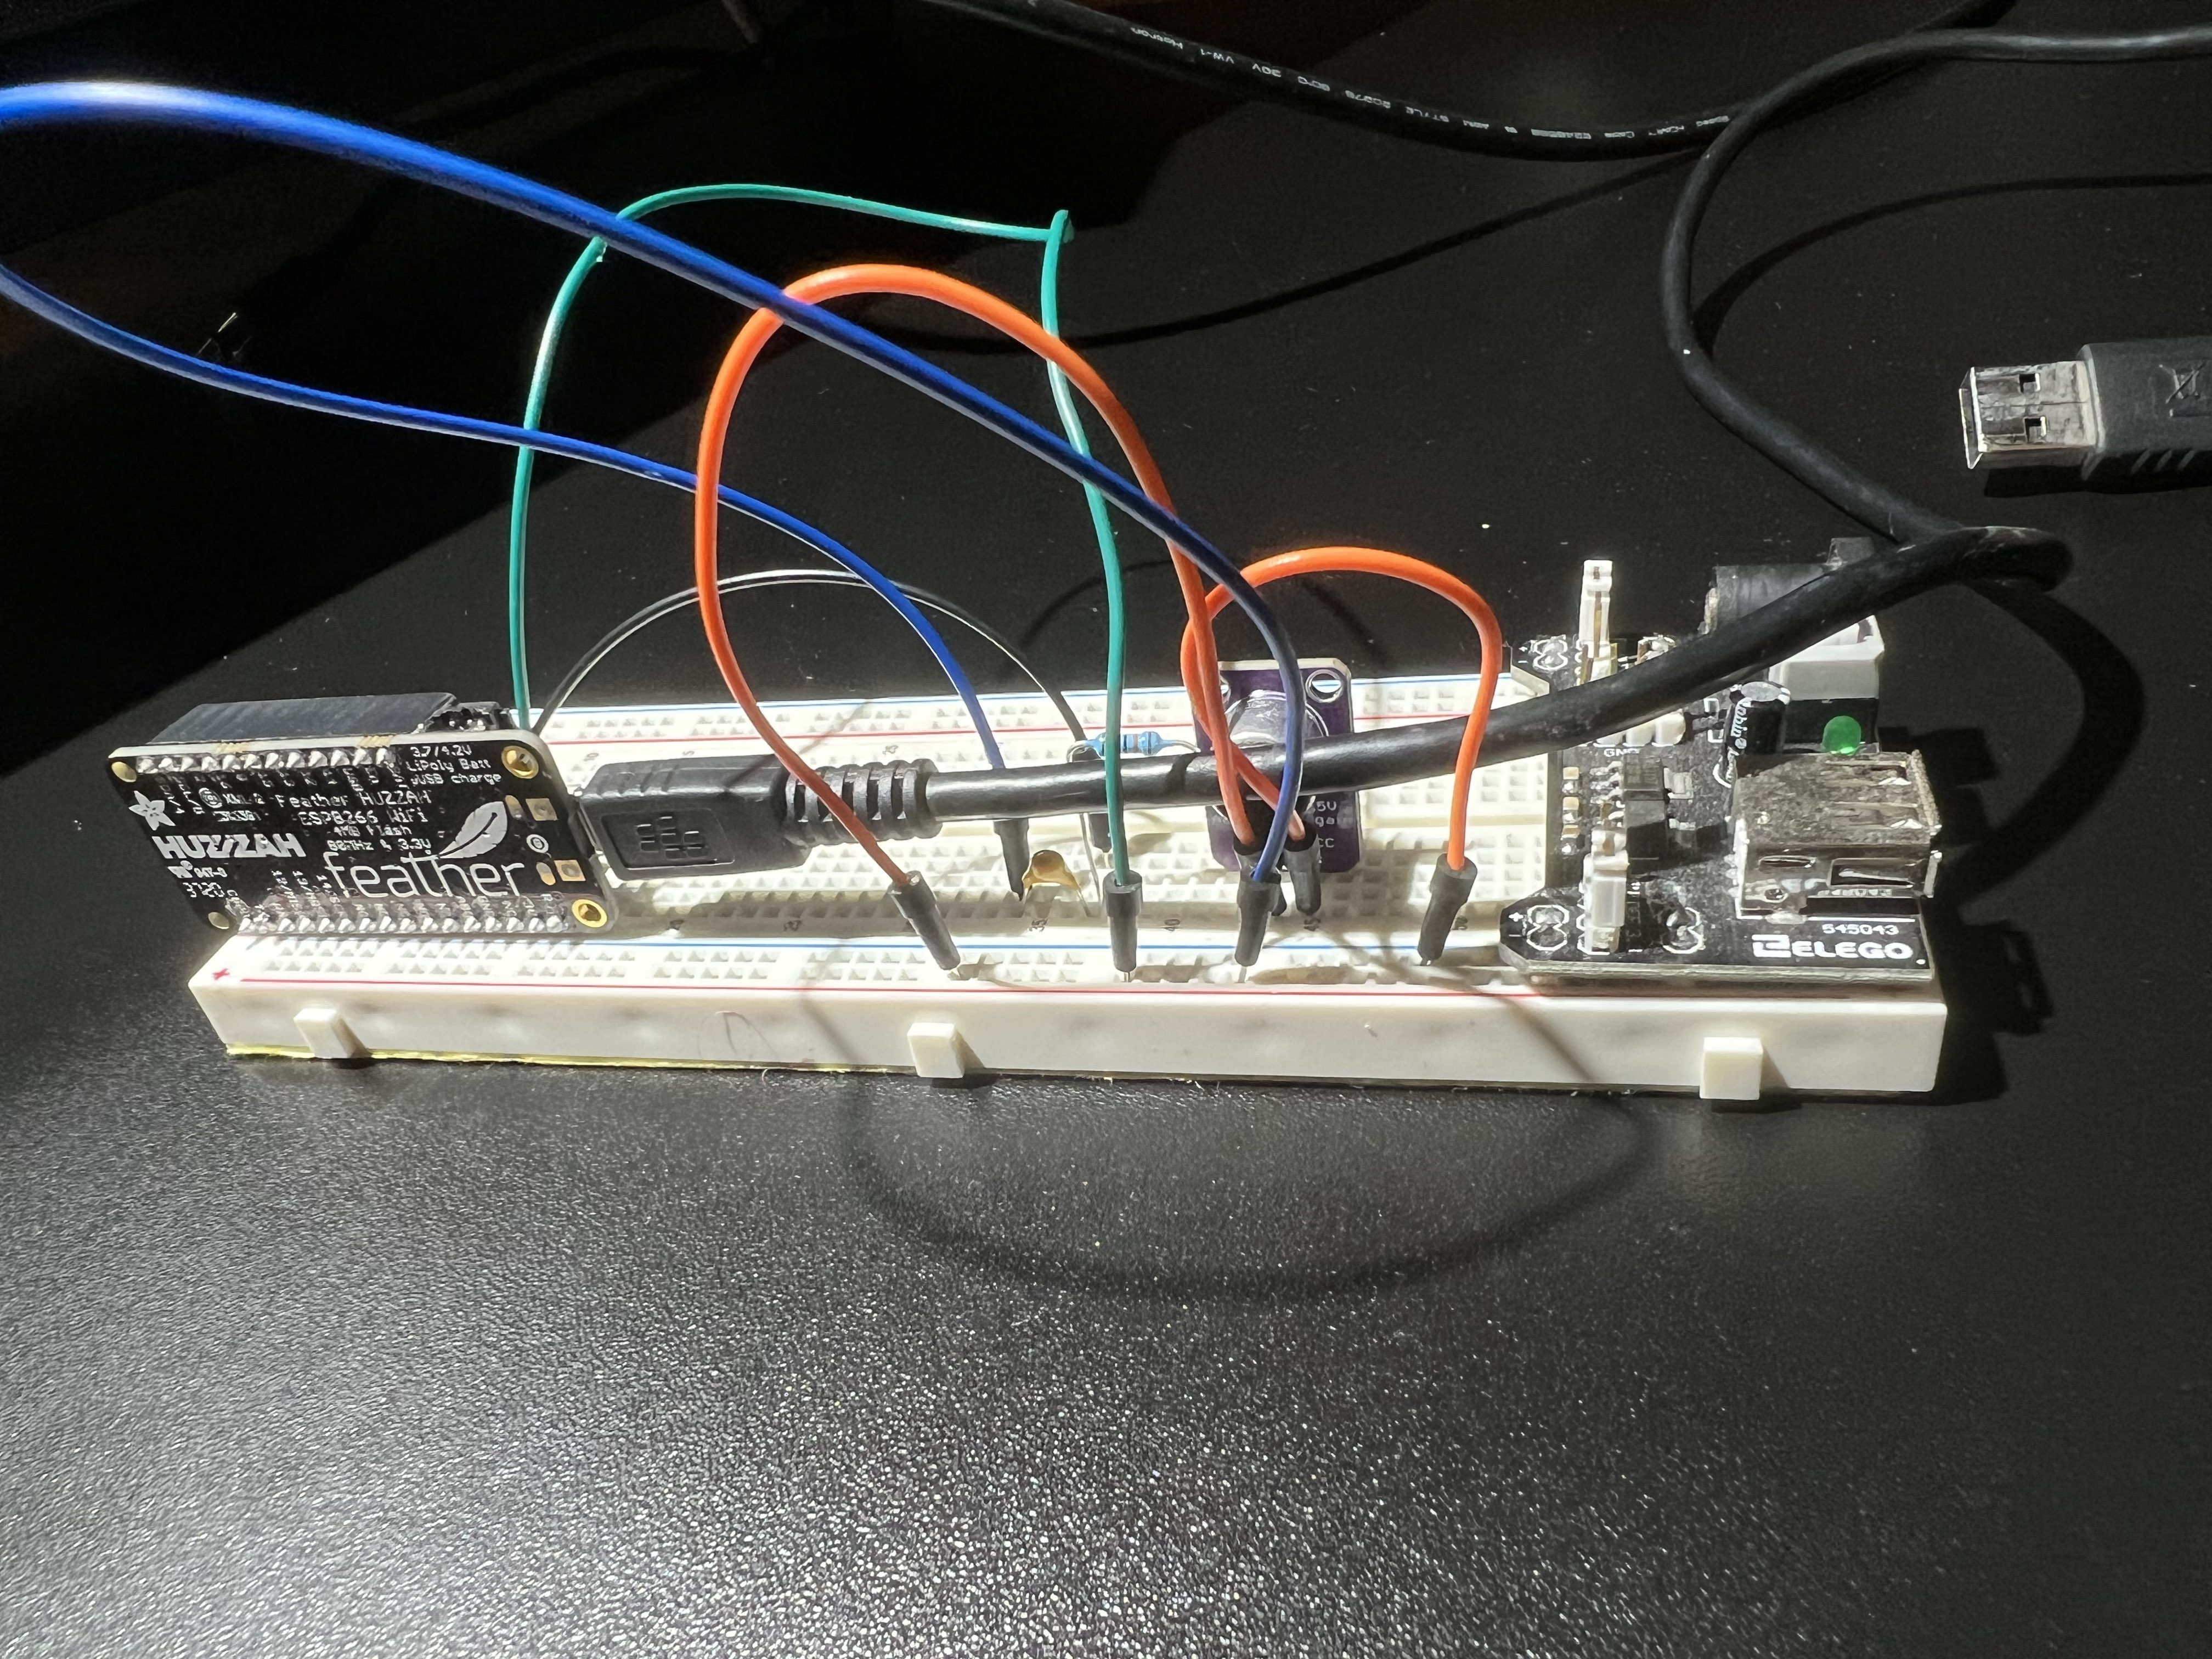
\includegraphics[width=0.8\textwidth]{sensing_node.jpg} % replace with your own image file
\caption{Prototype sensing node. A programmable gain microphone is connected to a 3.3V breadboard power supply. The output is filtered through an RC low-pass filter, and stepped down by a voltage divider to the 1V range of the ESP8266 ADC. The ESP8266 is connected by USB to a laptop for configuration through the serial port.}
\label{fig:sensing_node}
\end{figure}

\subsection{ESP8266}
	Each acoustic sensing node is implemented as an Adafruit Feather HUZZAH ESP8266 MCU which connects to a common WiFi network and communicates with the Raspberry Pi through web sockets. For my prototype, the ESP8266 is connected to my home router. 
	The EEPROM of the ESP8266 is flashed with the MicroPython runtime through a micro-USB cable connected to my laptop using the \textbf{esptool} CLI. Configuration of the ESP8266 can be done through the read-evaluate-print-loop (REPL) accessed through a serial port using PuTTY. MicroPython automatically executes the \textbf{boot.py} script in the ESP filesystem when the device is powered on, then executes \textbf{main.py}. Fig \ref{fig:PuTTY_REPL} shows the REPL through the serial port.
	
\begin{figure}[h]
\centering
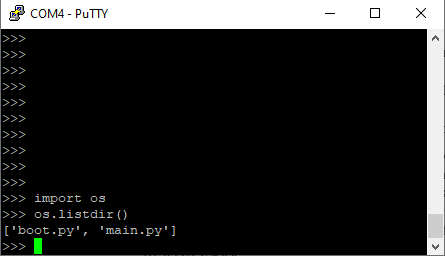
\includegraphics[width=0.8\textwidth]{PuTTY_REPL.png} % replace with your own image file
\caption{The MicroPython REPL on the ESP8266 is accessed through a serial port connection through PuTTY on a laptop for configuration.}
\label{fig:PuTTY_REPL}
\end{figure}
	
	In order to edit the scripts on the ESP8266, I use the \textbf{Ampy} command line tool created by Adafruit to modify the filesystem over the serial port. Ampy can be installed through \textbf{pip}, then commands can be issued to copy files over by specifying the serial port.
	I wrote a script \textbf{server.py} which is loaded onto the ESP. The script opens a web socket and listens for a connection from the Raspberry Pi, which . When the connection is made, the ESP begins sampling the ADC and stores the samples into a buffer. The buffer is sent over the connection to be recieved by the Raspberry Pi.


\subsection{Simulator}
	The effectiveness of localization based on acoustic signals depends on factors including:
	
\begin{itemize}
  \item Sensor noise
  \item Environment noise
  \item Sampling quantization
  \item Sensor and source geometry
  \item Sound speed
  \item Reverberation
\end{itemize}

	In order to test my localization algorithm under variation of these parameters, I created a simple simulator in Python to place sensors and sources spatially in the environment, add noise to the signal, simulate the sound propogating from source to each listening sensor, and visualize the localization result and error. The simulator uses the \textbf{Pygame} library to graphically represent the environment, shown in \ref{fig:simulator}.
	
\begin{figure}[h]
\centering
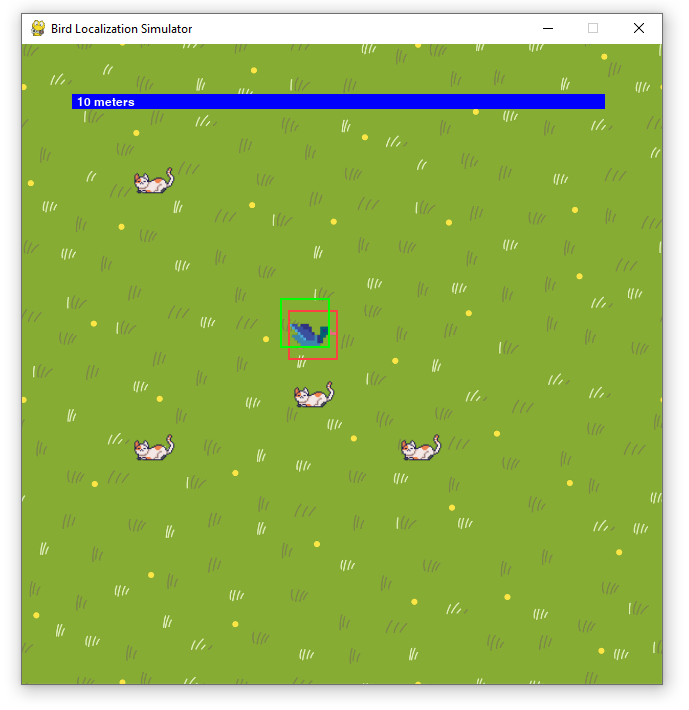
\includegraphics[width=0.8\textwidth]{simulator.png} % replace with your own image file
\caption{Graphical view of my bird localization simulator in Pygame. Sensing nodes are represented by cats, and the duck in the center represents the bird which is the sound source. The scale at the top shows the scale in meters. The red bounding box represents the true location of the bird and the green bounding box represents the estimate from the Chan-Ho algorithm.}
\label{fig:simulator}
\end{figure}

\subsection{Time-Difference Estimation (TDE)}
	To develop the TDE algorithm, I use the simulated time-shifted inputs, and apply the Generalized Cross-Correlation Phase Transform (GCC-PHAT) algorithm using the \textbf{Numpy} Python library. The peak of the digital correlation result between signals recieved at two nodes is used to determine the number of samples the signal is delayed by at one node compared to the other. Based on the sample rate, the time delay is determined.
	I iterate through all audio frames and compute TDE for each simulated node-pair. The resulting TDEs will be used in the localization algorithm to determine the localization result. I profile the execution time of the TDE algorithm, and write the output to a \textbf{csv} file for plotting.
	
\subsection{Fast Fourier Transform}
	The TDE algorithm I use is the Generalized Cross-Correlation Phase Transform (GCC-PHAT) algorithm. Which transforms the signal pair to the frequency domain using the Fast Fourier Transform. I profile the FFT algorithm provided by the Numpy library to evaluate the CPU time it requires, since the FFT accounts for the majority of required FLOPs in these algorithms. 
	
\subsection{Localization Estimate}
	The set of TDEs define a system of hyperbolic equations. When there are exactly 3 TDEs, the equations have one solution. With more than 3 TDEs, the matrix is overdetermined, and a least-squares method is necessary to make the final localization estimate. I use the Chan-Ho method. The Chan-Ho algorithm is heavy in linear algebra operations. For this project, I use the \textbf{Numpy} Python library to perform the matrix and vector operations, which under the hood, calls a compiled system BLAS library written in C located at \textbf{/usr/lib/aarch64-linux-gnu/blas}, and the compiled LAPACK library written in FORTRAN 77 located at {/usr/lib/aarch64-linux-gnu/lapack}. My profiling tests in the characterization process showed that these implementations take advantage of the Advanced SIMD architecture of the Cortex-A72 CPU for doing tensor operations, and vastly outperformed my best attempts at matrix multiplication in Rust.

% Results section
\section{Results}\label{sec:results}

\subsection{Characterization}

	The most important factor in getting reliable results for localization is understanding the error in the sensor data. The characterization of sensors is included in the estimator of the Chan-Ho algorithm, appearing in the covariance matrix of the TDoA estimates. 

\subsubsection{Microphone Noise}

	The results of my microphone tests described earlier are shown in Fig. \ref{fig:microphone}.

\begin{figure}[h]
\centering
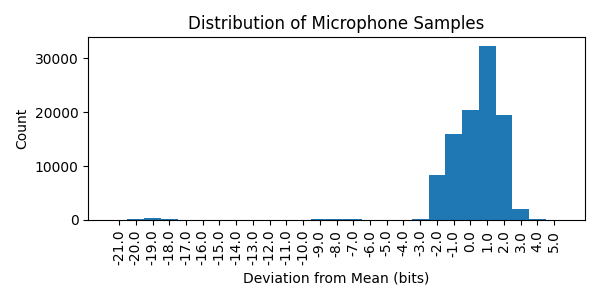
\includegraphics[width=0.8\textwidth]{microphone.png} % replace with your own image file
\caption{Histogram of 100,000 microphone samples from the ESP8266, sorted by deviation from mean sample value. The ADC has 10-bit precision, deviation is measured in 1-bit deviations.}
\label{fig:microphone}
\end{figure}

\subsubsection{GPS Spatial Precision}

	The collected GPS data is shown in Fig. \ref{fig:gps_distribution}.

\begin{figure}[h]
\centering
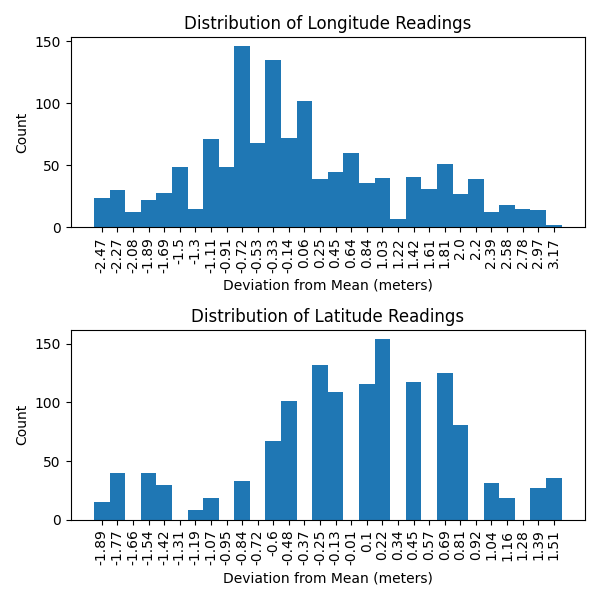
\includegraphics[width=0.8\textwidth]{GPS_distribution.png} % replace with your own image file
\caption{Histogram of 1,200 GPS readings of latitude and longitude, sorted by deviation from mean measured in meters.}
\label{fig:gps_distribution}
\end{figure}

\subsubsection{Classification Accuracy and Execution Time}

For the classification, I was able to run inference on a known bird species, and get a correct result, shown in Fig. \ref{fig:classification_result}.

\begin{figure}[h]
\centering
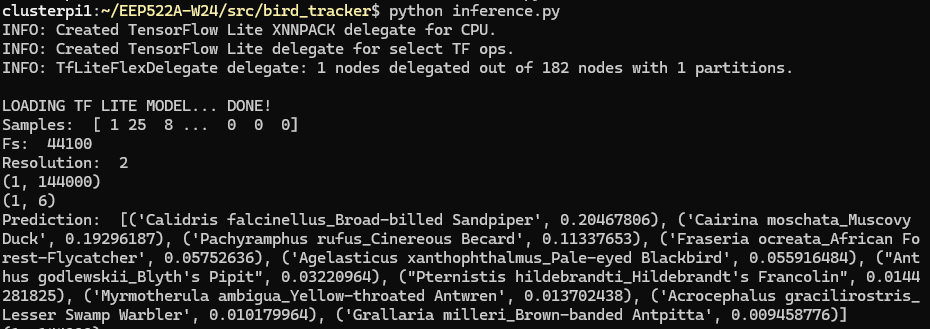
\includegraphics[width=0.8\textwidth]{classification_result.png} % replace with your own image file
\caption{Classification output for calidris falcinellus.mp3, the confidence score for the correct species is much greater than the next most probable class.}
\label{fig:classification_result}
\end{figure}

I profiled the time inference took to run on the Raspberry Pi, over several frames of audio, shown in Fig. \ref{fig:inference_times}.

\begin{figure}[h]
\centering
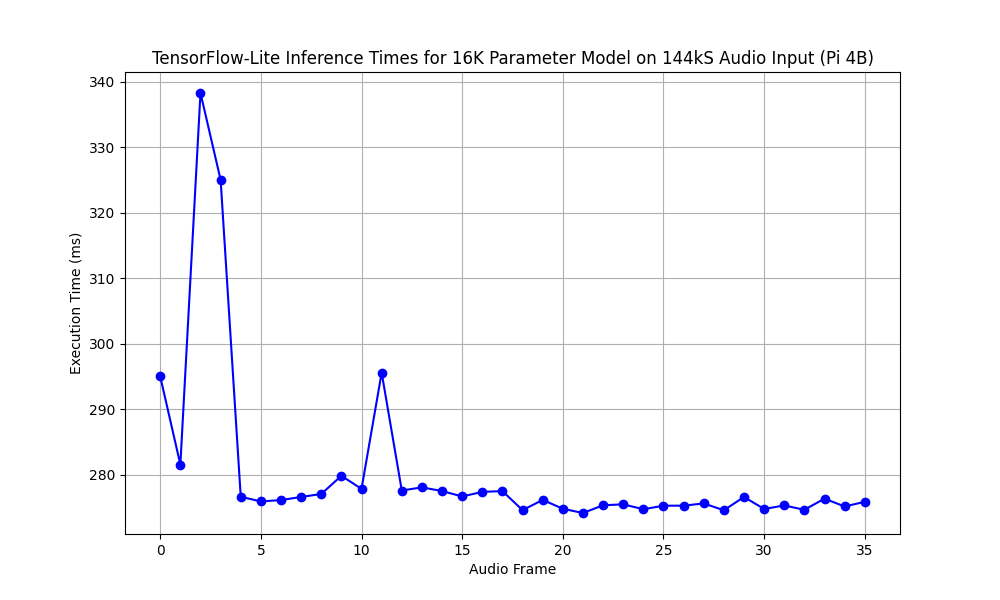
\includegraphics[width=0.8\textwidth]{Inference_times.png} % replace with your own image file
\caption{Profiled execution times for BirdNET classification inference using TensorFlow-Lite on the Raspberry Pi 4B.}
\label{fig:inference_times}
\end{figure}

\subsubsection{FFT and GCC-PHAT Execution Time}

I profiled the timing of the FFT and GCC-PHAT algorithms, shown in Fig. \ref{fig:fft_gcc_timing}.

\begin{figure}[h]
\centering
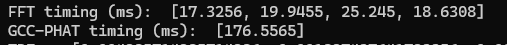
\includegraphics[width=0.8\textwidth]{fft_gcc_timing.png} % replace with your own image file
\caption{Profiled execution times several iterations of the FFT algorithm, and one iteration of the GCC-PHAT algorithm.}
\label{fig:fft_gcc_timing}
\end{figure}

\subsubsection{Chan-Ho Localization Accuracy and Execution Time}

The simulator results in Fig. \ref{fig:simulator} show that the localization estimate (green) is within a few hundred centimeters of the true location (red) of the bird.

% Discussion section
\section{Discussion}\label{sec:discussion}

\subsection{Performance}
	I found that my algorithm took a significant amount of the Raspberry Pi resources. The Pi can perform inference with the BirdNET model on a real-time input stream using about 10\% of the CPU time. The FFT algorithm also took a significant amount of CPU time. 
	The accuracy of the classification and localization was very good for a simulated initial prototype. Classification produced the correct bird species, and the localization algorithm using GCC-PHAT and Chan-Ho produced a localization result that was accurate to within a couple hundred centimeters for a 10 meter square problem space.

\subsection{Production}
	For small-scale hobbyist production, most of the pieces are there for someone to put a kit together. I would integrate the GPS, microphone, audio codec, and ESP8266 onto one circuit board with a battery and a 3D printable waterproof case. All the parts I used are very popular hobbyist components that are available in large quantities, nothing is specialty or unusual. I don't think there would be any supply chain issues. 
	There is a network and CPU time limit on how many sensing nodes can be supported by a single Raspberry Pi processing the data in real time. Past that limit, measures would have to be taken to properly buffer or discard signatures from nodes when there are back-to-back detections occuring.

\subsection{Self-assessment}
When I initially did my characterization of the board, I was interested in taking advantage of the compute capabilities of the GPU. I focused my attention on characterizing the capabilities of the GPU by running matrix multiplication on the GPU and comparing it to the CPU performance. I learned that the GPU was only capable of about 20\% the compute throughput of the CPU and that the software environment was very difficult to work with, since it has large or outdated dependencies depending on the method (Vulkan, V3DLib, qmlk6).

This drove me to understand how the CPU performs better than the GPU, by taking advantage of the ARM SIMD architecture, and specifically how Numpy outperforms both the GPU and my attempts with a faster language like Rust at linear algebra operations, by calling the LAPACK and BLAS compiled binaries optimized for the hardware under the hood.

In the area of compute, my characterization was key to doing the FFT, Least-squares, and inference with confidence that it was the correct method, which all use LAPACK and BLAS through Numpy.

\subsection{Future Improvements}
	The prototype I came up with falls short in multiple ways. The biggest one is that the ADC on the ESP8266 isn't sufficient for sampling at audio frequencies. In the future, I would use a dedicated audio codec which is designed for sampling at these rates. The audio codecs I was looking at are also capable of performing some DSP algorithms. It would be a significant improvement on the design if the FFT could be performed on specialized hardware to offload the work from the Raspberry Pi. 
	Another area of improvement is my simulator. Currently, the data pipeline doesn't support batched tests. I simply run it on one audio file, and print out the results to the console. A better simulator would allow me to run tests on a large assortment of data and input parameters and write the results to a log with useful statistics. I would also like to be able to simulate more physical parameters like reverberation and various noise sources. I just ran out of time for this project. 

\section{Conclusion}\label{sec:conclusion}

	In doing this project, and characterization, I learned a lot about the GPU and CPU on the Raspberry Pi, the vector processing capabilities of the Pi, and how Python (specifically Numpy) works to take advantage of processor architectures for matrix operations. I spent a large amount of time learning about the TensorFlow Lite environment to do inference on resource-constrained devices. I also read many papers to figure out how to implement the localization algorithm using GCC-PHAT and the Chan-Ho algorithm. I learned the MicroPython environment, and how to write a basic communication channel through web sockets, and proper buffering.
	I found simulating the problem visually to be a great help in debugging the algorithms, because it was obvious when the estimate was very far off. My immediate goals are to iterate on the simulator and begin processing larger datasets and vary more parameters. Overall, this project puts me in a very good position for my participation in the National Security Innovation Network's Good Vibration's challenge, where I am tasked with performing classification and localization of ground vehicles on a smaller Cortex-M4 MCU platform.

\paragraph{Note}
\textit{All my code and project files for this and future reports, can be found on my GitHub repository \cite{lybbert2024classwork}.}

% Bibliography from refs.bib
\bibliographystyle{plain}
\bibliography{refs}

\end{document}
